\documentclass[a4paper]{article}

\usepackage[swedish]{babel}
\usepackage[T1]{fontenc}
\usepackage[utf8]{inputenc}
\usepackage{graphicx}
\usepackage{array}
\usepackage{pbox}

\title{Projektplan DAT290 \\ \Large Larmsystem grupp 13}
\author{Filip Borg, Gustav Fåhraeus, Josef Karlsson,\\
            Erik Nilsson, Adam Thörnblom, Ben Wooldridge}
\date{2019-09-13}

\begin{document}
\maketitle
\pagenumbering{gobble}
\newpage

\tableofcontents
\newpage

\pagenumbering{arabic}


\section{SYFTE}
\label{sec:syfte}

Vi ska skapa ett larm för ett mindre företag. Syftet med larmet är att
\begin{itemize}
    \item Larma ifall en dörr är öppen för länge
    \item Upptäcka och förhindra inbrott
    \item Minimera inbrottets omfattning och kostnad

\end{itemize}
Rekomendationen enligt stöldskyddsföreningen är att ha ett larm
som är uppkopplat till en larmcentral. Därför ska vi skapa ett larm som är kopplat till en centralenhet,
 som övervakas dygnet runt.

\section{MÅL}
\label{sec:mål}

Målet med detta projekt är att med hjälp av ett antal mikrokontrollrar och periferienheter (bland annat rörelse- och vibrationssensor) konstruera ett larmsystem vars huvudsakliga uppgift är att varna när en dörr har varit öppen för länge. Varningen kommer att bestå i att en lysdiod tänds vid aktuell dörr efter en viss tid och att en signal, efter ytterligare en tid, sänds till centralenheten, varpå denna larmar med ljud. Från centralenheten skall användaren kunna ställa in ovan nämnda tidsfördröjningar samt larma och avlarma dörrarna. Systemet ska vara skalbart och således ha möjlighet att lägga till flera dörrar per enhet.

\section{BAKGRUND}
\label{sec:bakgrund}

Ett larmsystem av den typ som ska konstrueras använder olika typer av sensorer för att ta reda på om en dörr är öppen och om någon är i närheten. Denna information skickas till centralenheten för att vidta lämpliga åtgärder, alternativt hanteras lokalt vid varje dörrenhet.
Lämpliga åtgärder kan vara att tända en lysdiod, larma med ljud eller på annat sätt göra användaren uppmärksam på vad som har uppmätts.

\subsection{Tekniska förutsättningar}
\label{sec:tekniskaf}
Larmsystemet kommer att konstrueras av tre enheter som kommunicerar med varandra via en CAN-buss. Varje enhet består av en mikrokontroller (MD-407) och ett antal periferienheter, däribland en sensor som anger huruvida varje dörr är öppen, en rörelsesensor och en vibrationssensor. En av enheterna kommer att vara centralenhet och styra de två andra. Dessa två kommer vara koppplade till ett antal dörrar vardera med hjälp av olika sensorer.
I mjukvaran kommer ett eget protokoll tas fram och implementeras för kommunikation över CAN-bussen. Detta protokoll kommer styra hur enheter adresseras, anger sin prioritet och skickar meddelanden till varandra.



\section{SYSTEMÖVERSIKT}
\label{sec:systemö}
En priliminär systemöversikt över hårdvaran finns i Figur \ref{fig:hardware}.

Systemöversikten kommer med all sannolikhet förändras under projektets gång, den preliminära översikt är endast en utgångspunkt.
\begin{figure}[!ht]
	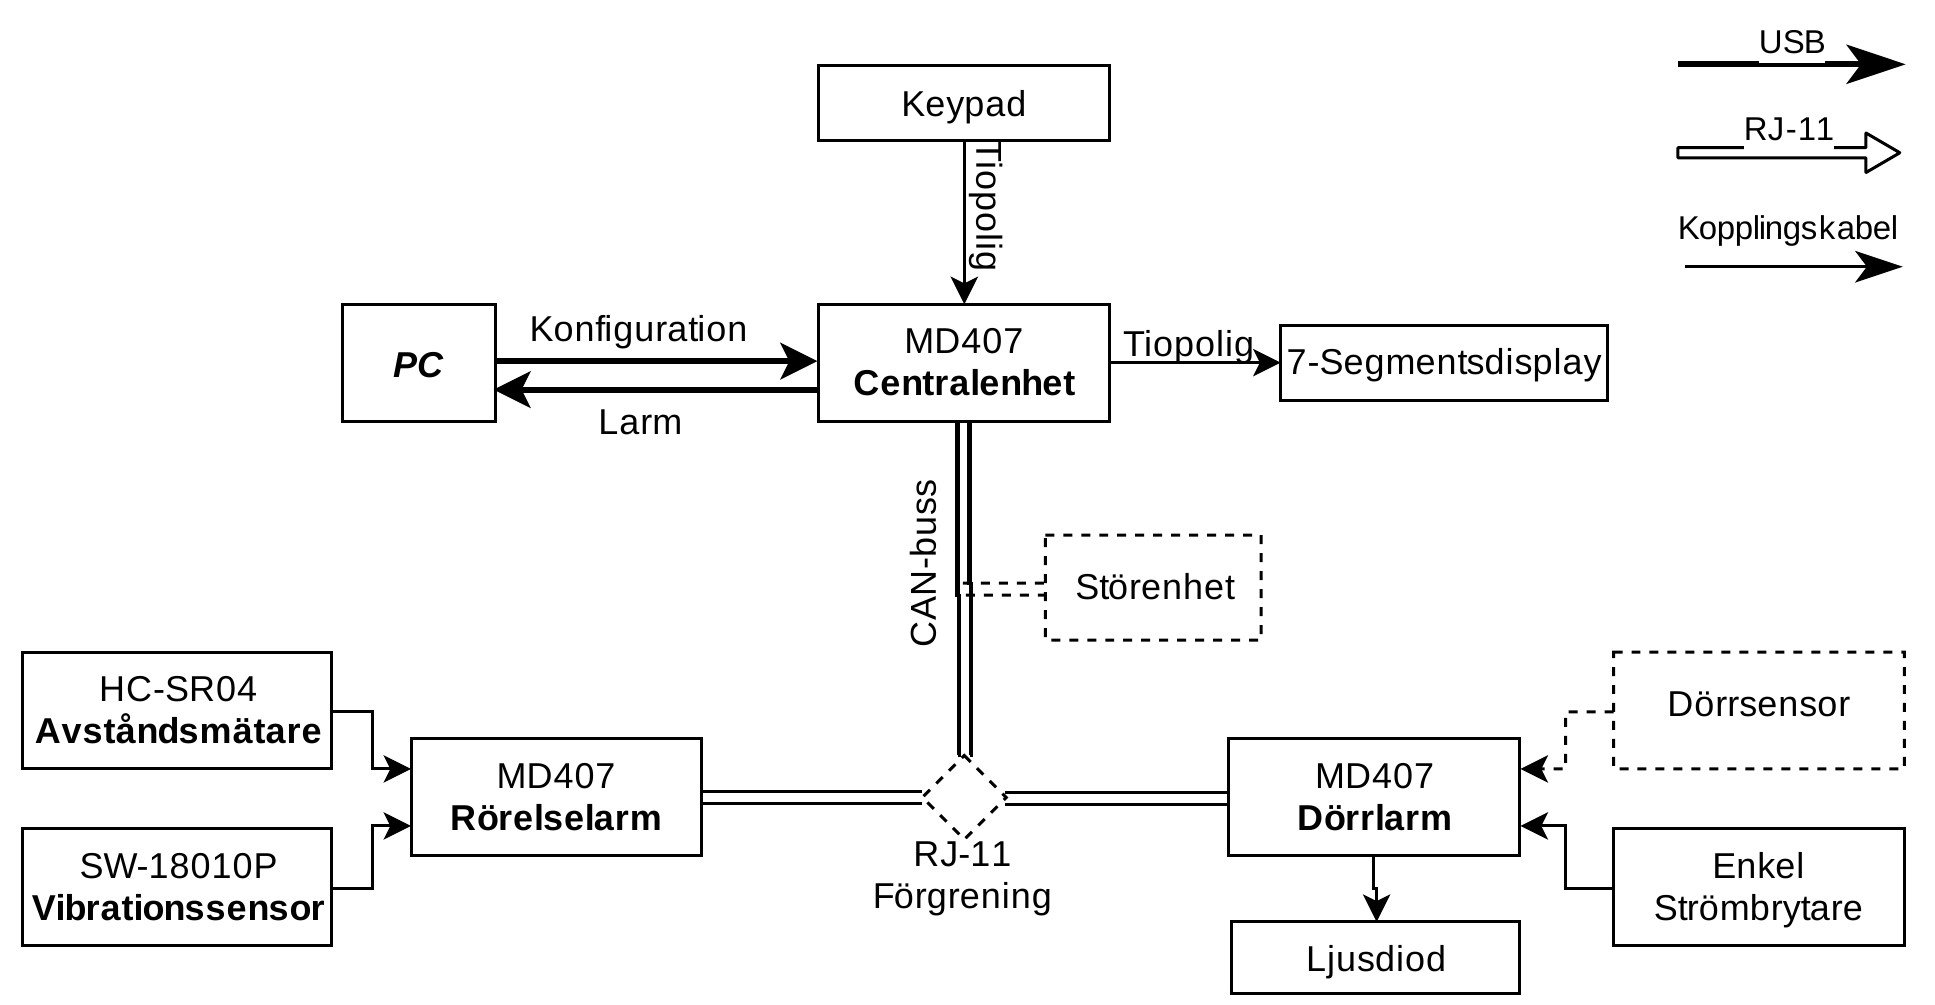
\includegraphics[width=1\textwidth]{figurer/Systemoversikt.jpg}
	\caption{Systemöversikt över hårdvaran}
	\label{fig:hardware}
\end{figure}

\section{RESURSPLAN}
\label{sec:resurs}

\begin{itemize}
    \item \textbf{Gruppledare:}
    \\
    Adam Thörnblom - (adam.thornblom@gmail.com)
    
    \item \textbf{Administrativt- och teknisk dokumentationsansvarig:} 
    \\
    Gustav Fåhraeus - (gusfah@student.chalmers.se)

    \item \textbf{Kodstandardansvarig:}
    \\
    Josef Karlsson - (effektgubben@gmail.com)

    \item \textbf{Testansvarig:}
    \\
    Filip Borg - (filipborg97@gmail.com) 

    \item \textbf{Resursansvarig:} 
    \\
    Ben Wooldridge - (benpontus17@gmail.com)

    \item \textbf{Planeringsansvarig:}
    \\
    Erik Nilsson - (ernilss@student.chalmers.se) 
\end{itemize}

Chalmers lokaler, och då främst diverse arbetsrum i EDIT-huset samt Idé-\\läran, kommer användas för gruppmöten och som arbetsyta.

Hårdvaran för projektet kommer att förvaras i grupprum 4211 i EDIT-huset. Hårdvaran som ska finnas tillgänglig är:
\begin{itemize}
    \item 3x MD407 kort 
    \item 1x Avståndsmätare (ultraljud), HC-SR04 
    \item 1x Vibrationssensor, "Flying-Fish" SW-18010P 
    \item 1x Keypad 
    \item 1x 7-segmentsdisplay 
    \item 2x 4-polig RJ-11 kabel (används för CAN-bussen) 
    \item 1x RJ-11 förgrening
    \item 2x Tiopolig flatkabel 
    \item 3x USB-kabel 
    \item 1x Kopplingsplatta
\end{itemize}

Kopplingskablar finns i projektrummet, dvs rum 4211 i EDIT-huset. Dörrsensor fås tillgång till genom att prata med handledare Rasmus Edvardsson.

Den nyaste fungerande versionen av mjukvaran som skrivs av gruppmedlemmarna fås tillgång till genom GIT där en gemensam repository för projektet har satts upp.

Arbete som sker utanför Chalmers kommer också bedrivas, både i grupp och enskilt. Detta kommer vara helt mjukvaruorienterat, om frågor skulle uppstå som kräver andra gruppmedlemmars uppmärksamhet så kommer dessa kunna nås via mail, eller via den gemensamma Messenger-gruppen som satts upp.

\section{MILSTOLPAR}
\label{sec:milstolpar}

I Tabell \ref{tab:milstolpar} finns de stora milstolparna för projektet.

	\begin{table}[htbp]
	\begin{tabular}{|c|l|c|c|}
		\hline
		Nr & BESKRIVNING & LV & DATUM \\ \hline \hline

		1 & Inlämning av projektplan & 2 & 2019-09-15 \\ \hline
		2 & Första kodraden i C & 2 & \\ \hline
		3 & \pbox{20cm}{Uppdelning av ansvarsområden \\ Perferienheter, Störenhet, Centralenheten} & 3 & \\ \hline
		4 & Till synes fungerande kommunikationsprotokoll & 3 & \\ \hline
		5 & Fungerande prototyp & 4 & \\ \hline
		6 & Påbörjande av Rapporten & 4 & \\ \hline
		7 & Påbörjande av extrauppgifter & 5 & \\ \hline
		8 & Inlämning av Rapportutkast 1 & 5 & 2019-10-06 \\ \hline
		9 & Inlämning av Oppositionsrapport &6 & \\ \hline
		10 & Inlämning av Rapportutkast 2 & 7 & 2019-10-20 \\ \hline
		11 & Grundsystemet helt färdigt & 7 & \\ \hline
		12 & Extrauppgifter helt färdiga & 8 & \\ \hline
		13 & Demo av systemet & 9 & \\ \hline
		14 & Inlämning av Slutrapport & 9 & 2019-11-03 \\ \hline
	\end{tabular}
	\caption{Milstolpar för projektet}
	\label{tab:milstolpar}
\end{table}

\section{AKTIVITETER}
\label{sec:sktiviteter}
Gruppens totala arbetstid på 1200 timmar planeras läggas ner enligt Tabell \ref{tab:aktiviteter}.
\newline

\begin{table}[b]
\begin{tabular}{|l|l|}
\hline
\multicolumn{2}{|c|}{\textbf{Aktiviteter}}                                   \\ \hline
\textit{Arbetsmoment}                                     & \textit{Tid (h)} \\ \hline
Föreläsningar                                             & 50               \\
Genomläsning av uppgift                                   & 10               \\
Initial-genomläsning av dokumentation för periferienheter & 10               \\
Framtagning av \LaTeX \,mallar                            & 5                \\
Projektledning                                            & 10               \\
Projektmöten                                              & 145              \\
Projektplan                                               & 35               \\
Kommunikationsprotokoll                                   & 30               \\
Programmering                                             & 600              \\
Kod-dokumentation granskning                              & 30               \\
Funktiontestning                                          & 20               \\
Prestandatestning                                         & 10               \\
Dokumentera testning                                      & 10               \\
Granskning \& Finputsning av kod                          & 30               \\
Yttre dokumentation (Slutgiltig systembeskrivning)        & 25               \\
Första utkast slutrapport                                 & 50               \\
Oppositionsrapporter                                      & 20               \\
Andra utkast slutrapport                                  & 20               \\
Förbered demonstration                                    & 20               \\
Demonstration                                             & 5               \\
Renskrivning slutrapport                                  & 30               \\
Kamratuppskattning                                        & 5                \\
Medverkansrapport                                         & 15               \\
Granskning medverkansrapport                              & 10               \\ \hline
\end{tabular}
\caption{Tidsplanering för projektet}
\label{tab:aktiviteter}
\end{table}

\section{TIDSPLAN}
\label{sec:tidsplan}

\begin{figure}[!ht]
	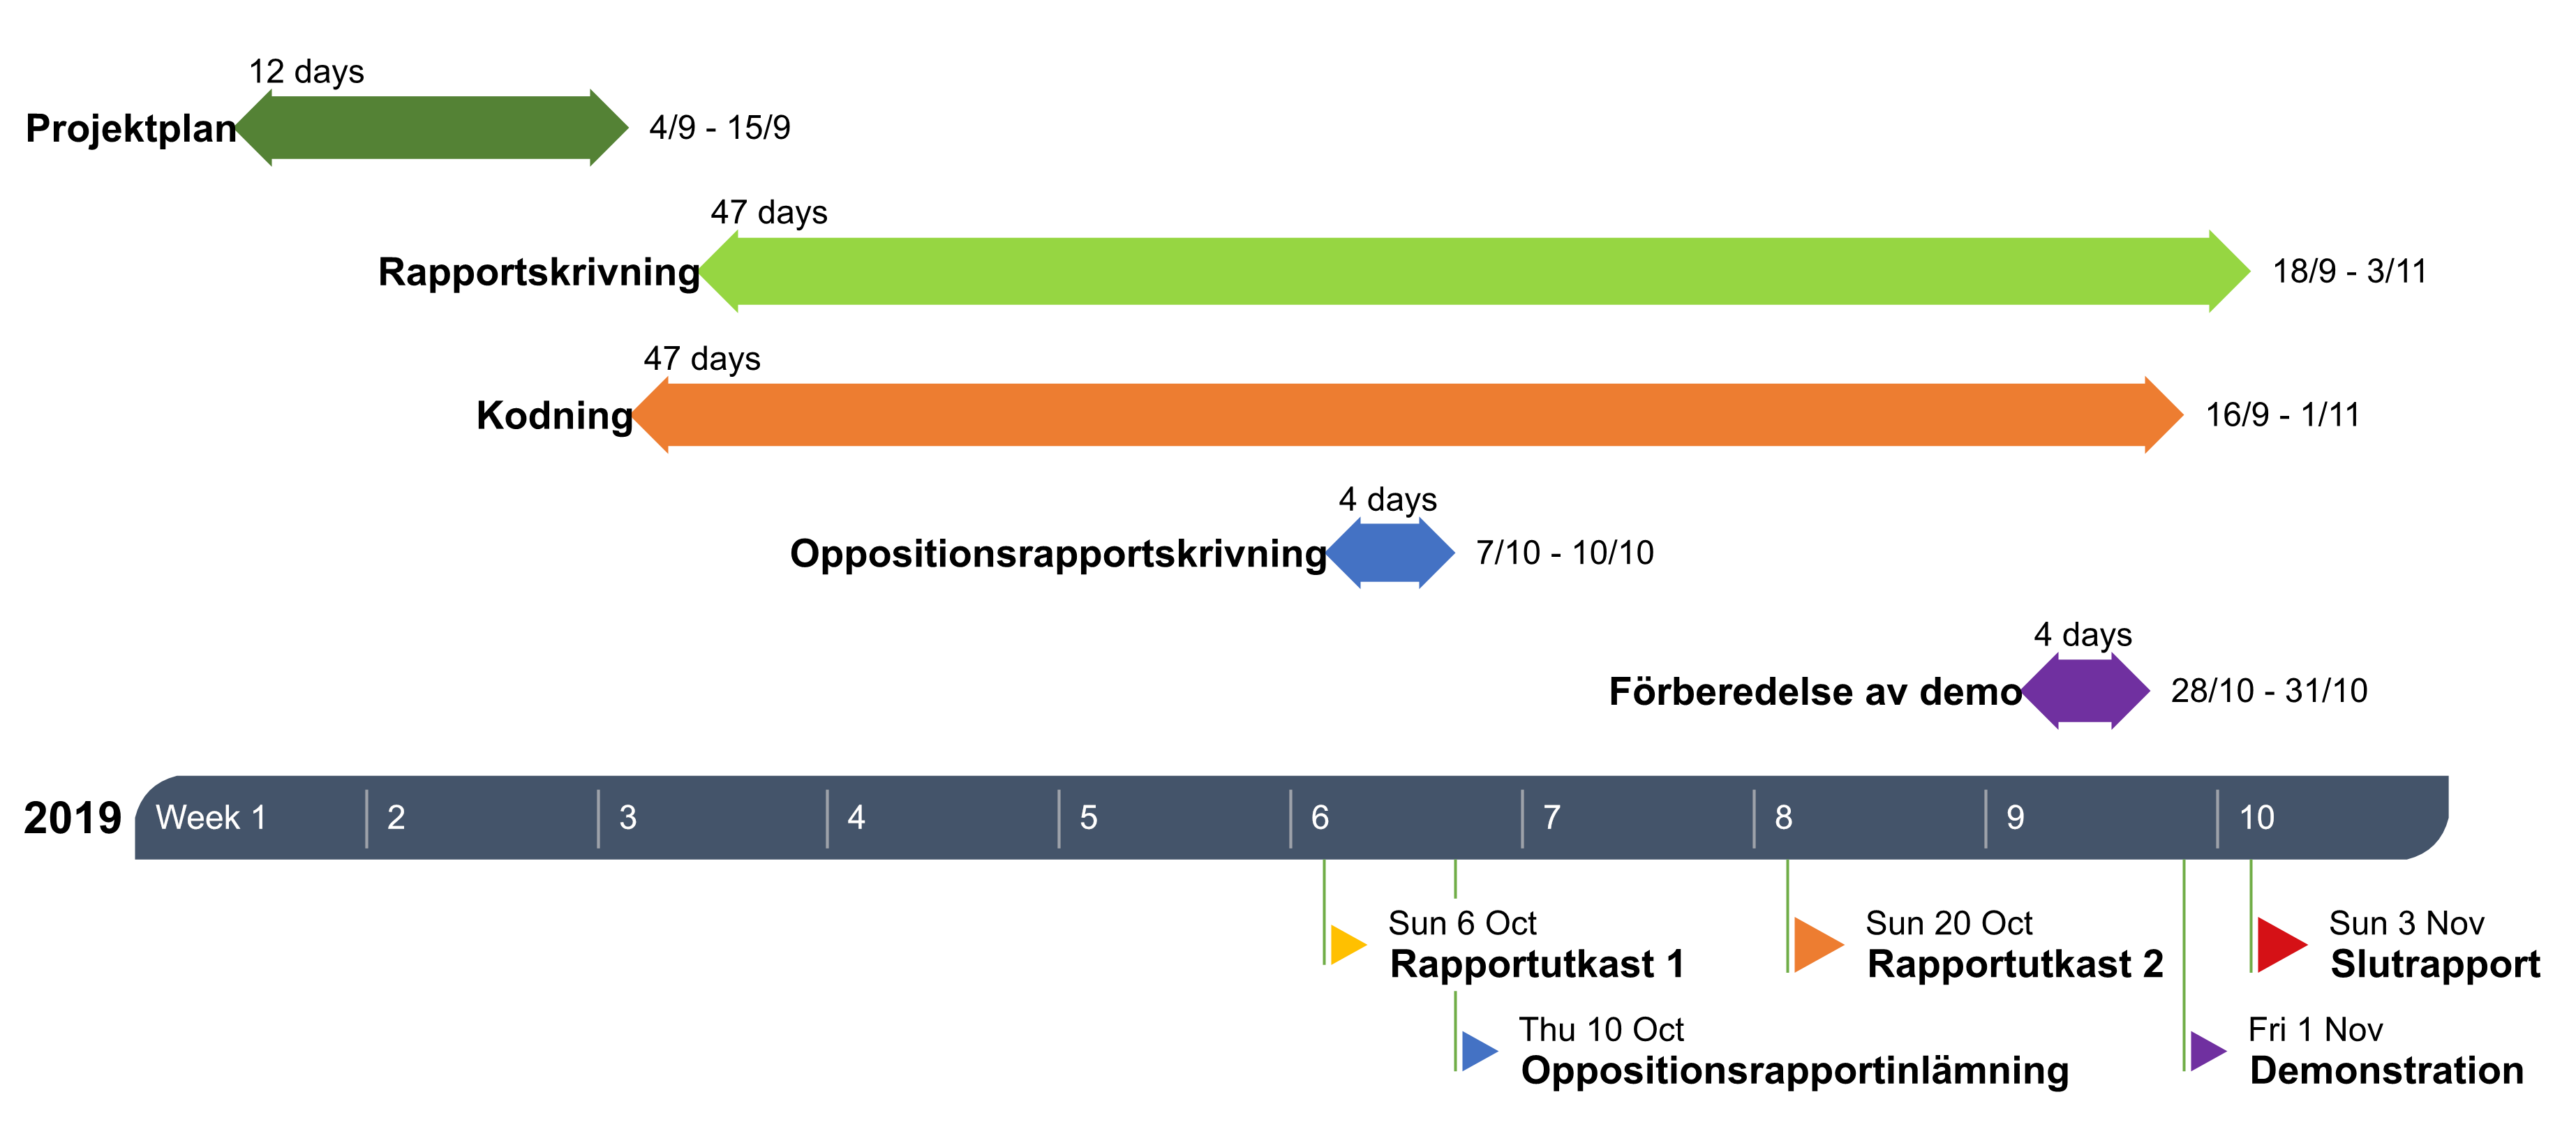
\includegraphics[width=1\textwidth]{figurer/Gantt.png}
	\caption{Ett Ganttschema med primära arbetsuppgifter och milstolpar}
	\label{fig:Gantt}
\end{figure}

\section{MÖTESPLAN}
\label{sec:mötesplan}

\textbf{Möten med handledare}
\begin{itemize}
	\item 2019-09-11 - prel. Tid: 09-10, Plats EG3505
	\item 2019-09-18 - prel. Tid: 09-10, Plats EG3505
	\item 2019-09-25 - prel. Tid: 09-10, Plats EG3505
	\item 2019-10-02 - prel. Tid: 09-10, Plats EG3505
	\item 2019-10-09 - prel. Tid: 09-10, Plats EG3505
	\item 2019-10-16 - prel. Tid: 09-10, Plats EG3505
	\item 2019-10-23 - prel. Tid: 09-10, Plats EG3505

\end{itemize}
\noindent
\textbf{Arbetsmöten}
\begin{itemize}
	\item 2019-09-11 - Tid 17:15-19:15, Plats EG3505
	\item 2019-09-  Måndagar 09:00-11:30 Torsdagar 08:45 - 09:45
	\item 2019-09-
	\item 2019-10-
	\item 2019-10-
	\item 2019-10-
	\item 2019-10-

\end{itemize}

\section{KOMMUNIKATIONSPLAN}
\label{sec:komm}

\begin{tabular}{|l|l|l|l|}
\hline
\multicolumn{1}{c}{\bfseries Vad} & \multicolumn{1}{c}{\bfseries När} & \multicolumn{1}{c}{\bfseries Till} & \multicolumn{1}{c}{\bfseries Hur} \\ \hline
Dagordning möte LV1 & 2019-09-02 & Alla & Canvas loggbok \\ \hline
Mötesprotokoll möte LV1 & 2019-09-03 & Alla & Canvas loggbok \\ \hline

Dagordning möte LV2 & 2019-09-11 & Alla & Canvas loggbok \\ \hline
Mötesprotokoll möte LV2 & 2019-09-13 & Alla & Canvas loggbok \\ \hline

Projektplan & 2019-09-15 & Lärarteam & Canvas Inlämning (Latex) \\ \hline

Dagordning möte LV3 & 2019-09-18 & Alla & Canvas loggbok \\ \hline
Mötesprotokoll möte LV3 & 2019-09-20 & Alla & Canvas loggbok \\ \hline

Dagordning möte LV4 & 2019-09-25 & Alla & Canvas loggbok \\ \hline
Mötesprotokoll möte LV4 & 2019-09-27 & Alla & Canvas loggbok \\ \hline

Dagordning möte LV5 & 2019-10-02 & Alla & Canvas loggbok \\ \hline
Mötesprotokoll möte LV5 & 2019-10-04 & Alla & Canvas loggbok \\ \hline

Rapportutkast 1 & 2019-10-06 & Lärarteam & Canvas Inlämning (Latex) \\ \hline

Dagordning möte LV6 & 2019-10-09 & Alla & Canvas loggbok \\ \hline
Oppositionsrapport & 2019-10-10 & Lärarteam & Canvas Inlämning (Latex) \\ \hline
Mötesprotokoll möte LV6 & 2019-10-11 & Alla & Canvas loggbok \\ \hline

Dagordning möte LV7 & 2019-10-16 & Alla & Canvas loggbok \\ \hline
Mötesprotokoll möte LV7 & 2019-10-18 & Alla & Canvas loggbok \\ \hline
Rapportutkast 2 & 2019-10-20 & Lärarteam & Canvas Inlämning (Latex) \\ \hline

Dagordning möte LV8 & 2019-10-23 & Alla & Canvas loggbok \\ \hline
Mötesprotokoll möte LV8 & 2019-10-25 & Alla & Canvas loggbok \\ \hline

Dagordning möte LV9 & 2019-10-30 & Alla & Canvas loggbok \\ \hline
Mötesprotokoll möte LV9 & 2019-11-01 & Alla & Canvas loggbok \\ \hline
Projektrapport & 2019-11-03 & Lärarteam & Canvas loggbok \\ \hline
Kamratuppskattning och medverkansrapport & 2019-11-03 & Lärarteam & Canvas Inlämning (Latex) \\ \hline



\end{tabular}
\\ \\
Kommunikation kommer även ske internt via en gruppchatt på Messenger-appen, och via logsen på GitHub.
\\

\section{KVALITETSPLAN}
\label{sec:kval}

För att säkerställa kvaliteten hos systemet ska tester kontinuerligt utföras och analyseras. Dessa tester ämnar att verifiera funktionalliteten hos mjukvara, hårdvara, delsystem samt det färdiga systemet. Vid utförande av test fylls mallen nedan i, det resulterar i ett protokoll som sedan sparas som verifikation. Målet med dessa protokoll är att man utan sakkunskap ska kunna skapa sig en överblick av att systemet fungerar som det ska.

\begin{description}
	\item[Utfört av] Namn på de involverade samt datum för testets utförande.

	\item[Komponent] Vilken del av systemet testas?

	\item[Testsyfte] Vad ska testet visa? Är testet till följd av tidigare test?

	\item[Hjälpmedel] Lista hjälpmedlen som användes i samband med testet.

	\item[Utförande] Hur ska testet utföras?

	\item[Resultat] Vad är testresultatet? Hittades några buggar?

	\item[Analys] Vad innebär testets resultat? Behövs fler test av komponenten? Behö-
	ver andra komponenter testas ytterligare, och i så fall hur?
\end{description}

\section{SPELREGLER}
\label{sec:spelregler}

För förhindrande av misskötsel i projektgruppen införs ett straffsystem kallat ”Påföljdsfikan”. Påföljdsfikan fungerar så att efter en gruppmedlems misskötsel skall hen nästa sammankomst bjuda på fika för $S_{namn} = S_{namn} + k_{namn}*25$ kr omm $k_{namn}>1$, där $k_{namn}$ och $S_{namn}$ är varje individuella gruppmedlems kakfaktor, som ökas efter varje misskötsel men kan ej minskas utan benådning, respektive kakskuld som ackumuleras fram tills dess att gruppmedlemmen betalar tillbaka den. Initialvärdet för $S_{namn}$ och $k_{namn}$ är: $S_{namn}=k_{namn}=0.$\\ \par
Punktlista över straff:
\begin{itemize}
	\item 5–10 min sen till möte, $k_{namn} = k_{namn} + 0.5$
	\item 10-30 min sen till möte, $k_{namn} = k_{namn} + 1$
	\item 30+ min sen till möte, $k_{namn} = k_{namn} + 1.5$
	\item Kommer ej till mötet, $k_{namn} = k_{namn} + 2$
	\item Ej klar med veckans uppgifter eller slarvigt gjorda, $k_{namn} = k_{namn} + 1$
	\item Ej påbörjat veckans uppgifter eller icke klar och slarvigt gjorda uppgifter, \indent $k_{namn} = k_{namn} + 2$
	\item Ödeläggelse av git repository, $k_{namn} = k_{namn} + 3$
\end{itemize}
\par
Gruppmedlemmar kan benådas straff omm de har en ursäkt som godkänts av en annan gruppmedlem senast 30 minuter i förväg eller majoriteten av resterande medlemmar (3/5) godkänner en försenad ursäkt. $S_{namn}$ och $k_{namn}$ kan minskas, ej under 0, vid överlägsen majoritetröst (4/5) från resterande medlemmar.



%För referenser
%\bibliographystyle{IEEEtran}
%\bibliography{referenser}
\end{document}
